
\section{Data Preparation}
Kaggle is a public platform which provides various types of data for research purpose. The dataset 'foodRecSys-V1' used in this thesis is received from Kaggle \cite{48}. This dataset consists of three files. The 'core-data\_recipe.csv' file has all information about recipes such as 'recipe\_id', 'recipe\_name', 'image\_url', 'ingredients', 'cooking\_directions', 'nutritions' as shown in \autoref{fig:raw_recipes_head}. It has $45630$ recipes with $6$ columns as per \autoref{fig:raw_recipes_shape}.

\begin{figure}[H]
	\centering
	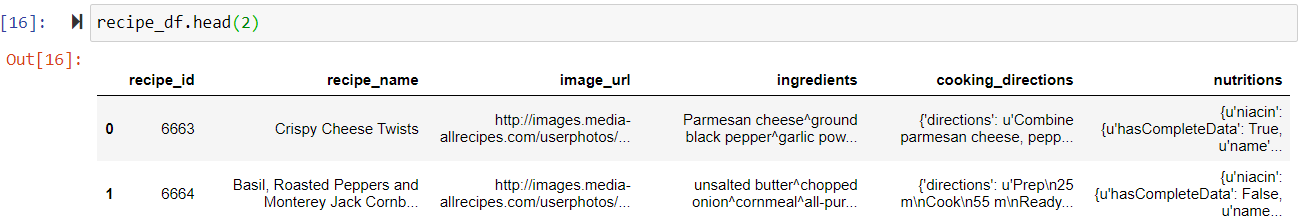
\includegraphics[width=1.0\linewidth]{raw_recipes_head}
	\caption{Raw Recipe Data}
	\label{fig:raw_recipes_head}
\end{figure}

\begin{figure}[H]
	\centering
	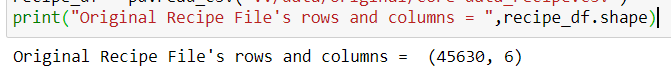
\includegraphics[width=1.0\linewidth]{raw_recipes_shape}
	\caption{Rows and Columns of original recipe's file}
	\label{fig:raw_recipes_shape}
\end{figure}

\noindent The other two files 'core-data-train\_rating.csv' and 'core-data-test\_rating.csv' provide user interactions with recipes. User interaction refers to a record in the file such as a user has given a rating to a recipe as depicted in \autoref{fig:raw_ratings_head}. These two files are combined and formed a single file that has all user interactions.  It has $960386$ users-recipes interactions and $4$ columns, 'user\_id', 'recipe\_id', 'rating', 'dateLastModified' as shown in
 \autoref{fig:original_interactions_shape}.

\begin{figure}[H]
	\centering
	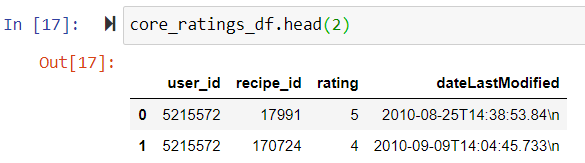
\includegraphics[width=0.8\linewidth]{raw_ratings_head}
	\caption{Raw User-Interaction Data}
	\label{fig:raw_ratings_head}
\end{figure}

\begin{figure}[H]
	\centering
	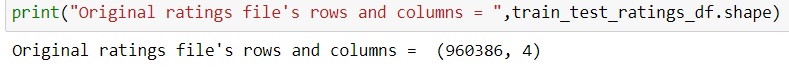
\includegraphics[width=1.0\linewidth]{original_interactions_shape}
	\caption{Rows and Columns of original user-recipes interactions }
	\label{fig:original_interactions_shape}
\end{figure}  


\subsection{Features Extraction}
A content-based filtering algorithm relies on the contents of the items. In our dataset, recipes are items that are rated by users. To recommend any recipe for a user, it is important to understand the features of the recipe that are relevant for a user. This thesis considers 'Ingredients', 'Cooking Method', 'Calories' and 'Diet Labels' features to find similarities between recipes.

\subsubsection{Ingredients Extraction}
The recipe's data received from Kaggle has the ingredients column in a clean format at a certain level. To get a single ingredient for each recipe, the "NLTK" library has been used. It tokenizes sentences into words. Raw ingredients data has many words that are irrelevant in predicting similarity between ingredients such as 'white' from 'white eggs', 'frozen', 'thawed', 'piece'. Such custom keywords are added in a recipe\_stopwords list and removed them from ingredients to make ingredients very specific. The difference between raw ingredients and cleaned ingredients is illustrated in \autoref{fig:raw_ingredients} \autoref{fig:clean_ingredients}. Irrelevant words such as 'thawed' and 'white' present in the first column of the pre-processed ingredients column have been removed in post-processed ingredients.

\begin{figure}[H]
	\centering
	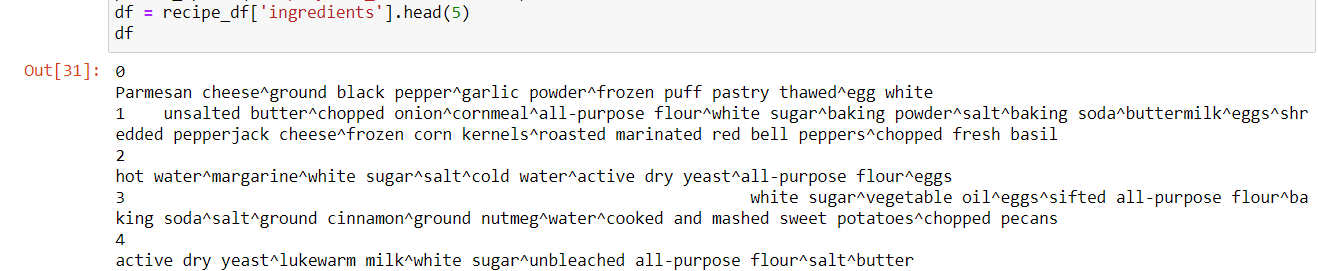
\includegraphics[width=1.0\linewidth]{raw_ingredients}
	\caption{Pre-Processed Ingredients }
	\label{fig:raw_ingredients}
\end{figure}  


\begin{figure}[H]
	\centering
	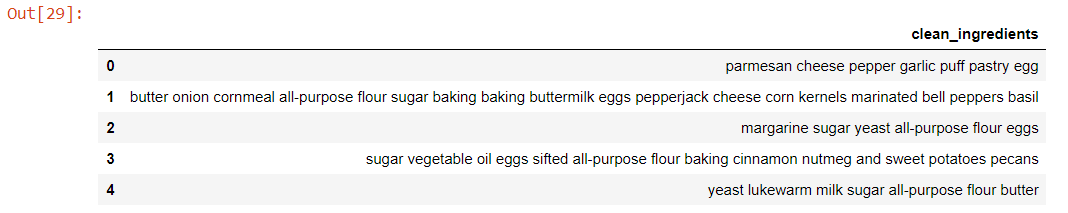
\includegraphics[width=1.0\linewidth]{clean_ingredients}
	\caption{Post-Processed Ingredients }
	\label{fig:clean_ingredients}
\end{figure}  

\subsubsection{Cooking Method Extraction}
Ingredients are most significant in measuring the similarity between recipes but instead of only ingredients, Wang et al. [49] represented the recipes as graphs which are built on ingredients and cooking directions can be used to easily aggregate dishes. 
The University of Minnesota has predefined glossary of cooking methods \cite{50} that has $74$ cooking methods such as 'bake', 'steam', 'fry' just to name a few. Recipes dataset of this thesis has a 'cooking\_direction' column that contains the method of cooking. It is a set of sentences that provides all instructions for a recipe as shown in \autoref{fig:cooking_directions}.
\begin{figure}[H]
	\centering
	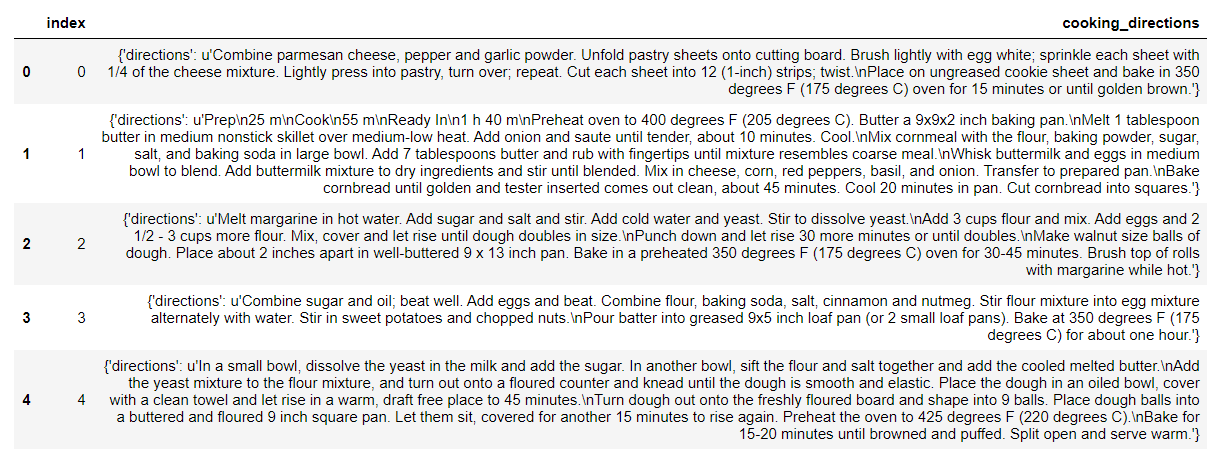
\includegraphics[width=1.0\linewidth]{cooking_directions}
	\caption{Cooking Directions }
	\label{fig:cooking_directions}
\end{figure}  

\noindent To get a cooking method from cooking direction, 'NLTK Processing' is performed on 'cooking\_direction' column.  First step of this processing is to convert set of instructions into words. Conversion of sentences to words is done by using 'NLTK Tokenizer.' Next step is to remove 'stop words' from sentences. In natural language processing, stop words are refers to words that do not have meaningful information such as 'a', 'and', 'an', 'the'. These words are considered as noisy data and can be ignored. These stop words are downloaded from the 'NLTK' library. Result is a list of keywords of cooking methods and ingredients. The common words from this result and predefined glossary of cooking methods are extracted and considered as cooking methods used in the associated recipe. The list of cooking methods used in associated recipes is depicted in \autoref{fig:cooking_methods}.
\begin{figure}[H]
	\centering
	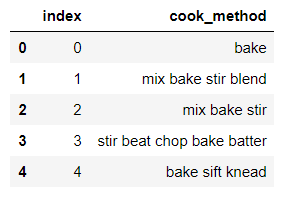
\includegraphics[width=0.5\linewidth]{cooking_methods}
	\caption{Cooking Methods }
	\label{fig:cooking_methods}
\end{figure}  

\subsubsection{Calories Extraction}
A calorie is a unit of an energy. Calories in any food refers to the energy people get by consuming food. Recipe dataset has 'nutrition' column. For each recipe, nutrition values are specified with quantity. For example, 'Crispee Cheese twists' recipe has 121 calories as depicted in  \autoref{fig:nutritions}. This information is stored in the nested dictionary. After extracting calorie's information it is stored in the 'calories' column as showin in \autoref{fig:calories}.
\begin{figure}[H]
	\centering
	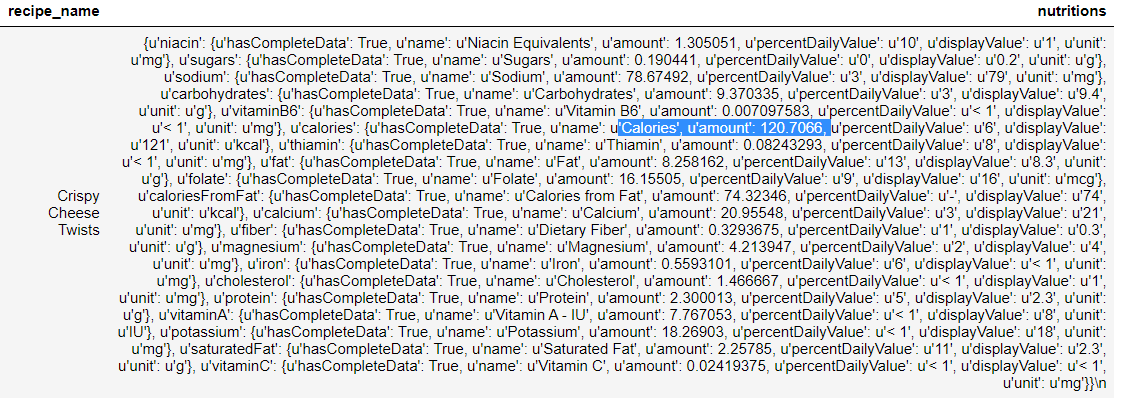
\includegraphics[width=1.0\linewidth]{nutritions}
	\caption{Recipe - Nutrition }
	\label{fig:nutritions}
\end{figure}  

\begin{figure}[H]
	\centering
	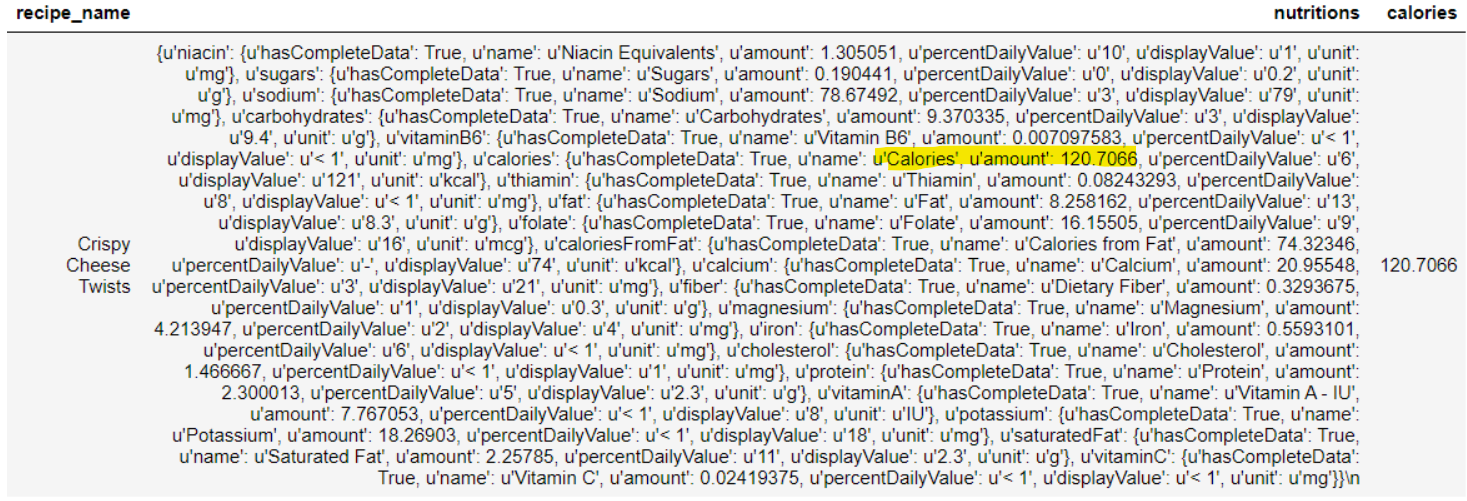
\includegraphics[width=1.0\linewidth]{calories}
	\caption{Recipe - Calories }
	\label{fig:calories}
\end{figure}  

\subsubsection{Diet Labels Extraction}
According to U.S. Food and Drug Administration (FDA) \cite{51}, \%DV is the percentage of the Daily Value for each nutrient in a serving of the food. Percentage Daily Value can inform if a serving of food is high or low in a nutrient. The general guide is 5\% DV or less of a nutrient per serving is considered low and 20\% DV or more of a nutrient per serving is considered high. From this information, recipes are broadly divided into five categories such as \textbf{"highprotein"}, \textbf{"highfiber"}, \textbf{"lowfat"}, \textbf{"lowcarb"}, \textbf{"lowsodium"} and \textbf{"balanced"}. If \%DV value is less than 5\% then recipe will fall under low nutrition label category otherwise in high nutrition label category. For example, \autoref{fig:diet_labels} illustrates that recipe 'Crispee Cheese Twist' has percentage daily value for carbohydrates is $3$ and for sodium is $3$ that is less than 5\%. Hence 'Crispee Cheese Twist' will fall under 'Low-Carb' and 'Low-Sodium' category.
\begin{figure}[H]
	\centering
	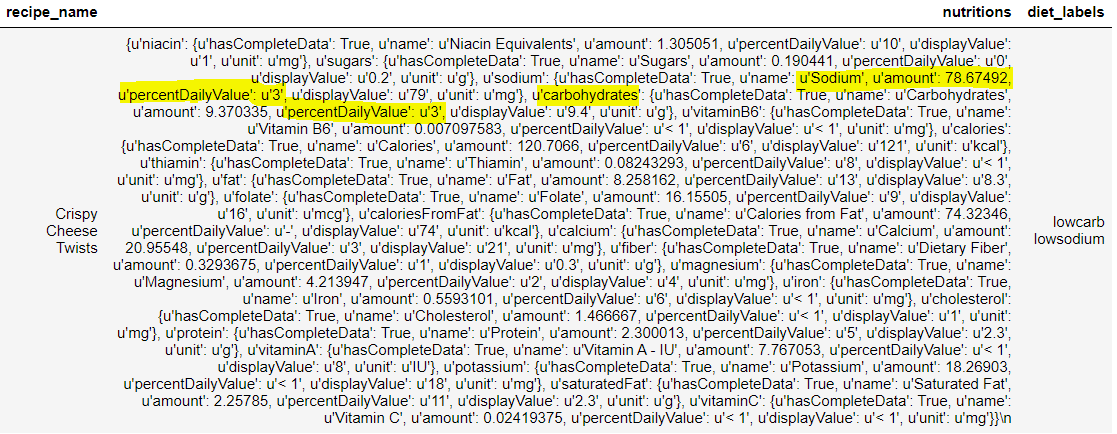
\includegraphics[width=1.0\linewidth]{diet_labels}
	\caption{Recipe - Diet Labels }
	\label{fig:diet_labels}
\end{figure}  

\subsubsection{User Information}